\graphicspath{{}{theory/}}


Neutrinos provide the most compelling evidence for physics beyond the SM. In this chapter we explore why and discuss some of the most important properties of neutrinos for their experimental study.

Neutrinos are purely weakly interacting fields

Neutrinos -- Pauli + Madame Wu + Freinberg numus + Lederman

\section{Oscillations}

\section{Sources}

To find a source of neutrinos, all we have to do is to look for environments where the Weak force is prominently manifested. A natural candidate, as we have seen in the discovery of the neutrino, are nuclear reactors. Fortunately, the list does not stop there. We now discuss in some detail some of the most important sources of neutrinos used in modern experiments.

\paragraph{Low energies (meV $\to$ MeV)}

\paragraph{Medium energies (MeV $\to$ 100's of GeV)}

\paragraph{High Energies (100's of GeV $\to$ EeV)}


\section{Scattering}

Neutrino cross sections are an invaluable observable to understand the Weak force and to search for new physics. 

\begin{figure}
%  \includegraphics[width=\textwidth]{}
\end{figure}



\section{Mass mechanisms}

\begin{figure}[t]
\centering
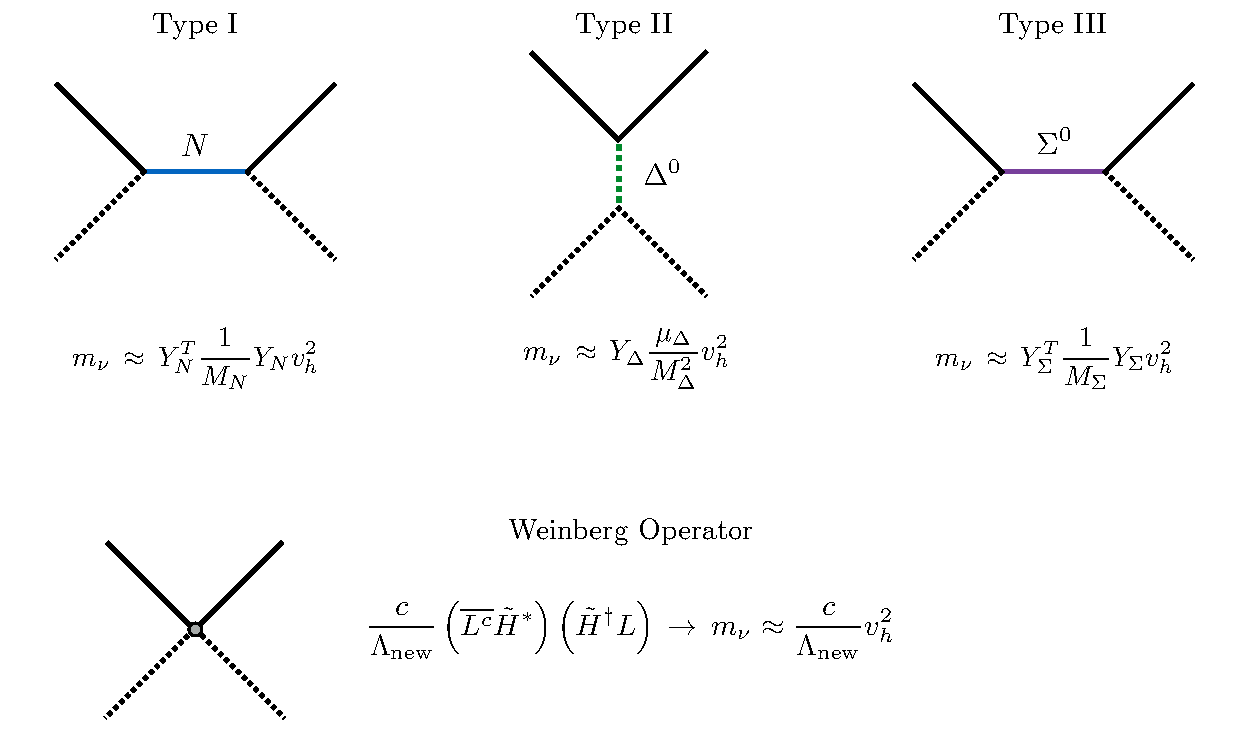
\includegraphics[width=\textwidth]{seesaw_mechanisms.pdf}
\caption[The tree-level UV completions of the Weinberg operator.]{The only three UV completions of the $d=5$ Weinberg operator with their respective contributions to light neutrino masses.\label{fig:seesaw_mechanisms}}
\end{figure}


In \reffig{fig:seesaw_mechanisms}, we show these unique tree-level completions of the Weinberg operator.

For a review on low-scale models see \cite{Boucenna:2014zba}.

\subsection{Conventional seesaws}

\subsection{Low scale seesaw variants}

\subsection{Radiative masses}

The most straightforward extension of the SM which can generate neutrino masses at loop level is perhaps the so-called Zee-Babu model.